% ============================================================================
% LaTeX figure blocks for:
% "Riding out the Dunkelflaute: A techno-economic assessment of SMR and
%  Gen-IV nuclear coupling with high-share renewables in the German power
%  system"
%
% Source of truth: RESULTS_FINAL.md (authoritative, 2026-07-07)
% Scenario names used consistently: Base, Dunkelflaute, SMR, MSR, LFR
%
% Usage: requires \usepackage{graphicx} in the preamble.
% Figures marked "full-width" assume \textwidth ~= 7.5-8in (or use figure*
% in a two-column layout). Figures marked "single-column" fit a 6.5in column.
% PDF versions are vector and preferred for LaTeX compilation (pdflatex/xelatex);
% PNG (300 dpi) is provided as a fallback / for non-PDF workflows.
% ============================================================================

% ---------------------------------------------------------------------------
% Figure 1 — Modelling workflow and scenario structure
% Full-width, portrait orientation (tall figure)
% ---------------------------------------------------------------------------
\begin{figure}[htbp]
    \centering
    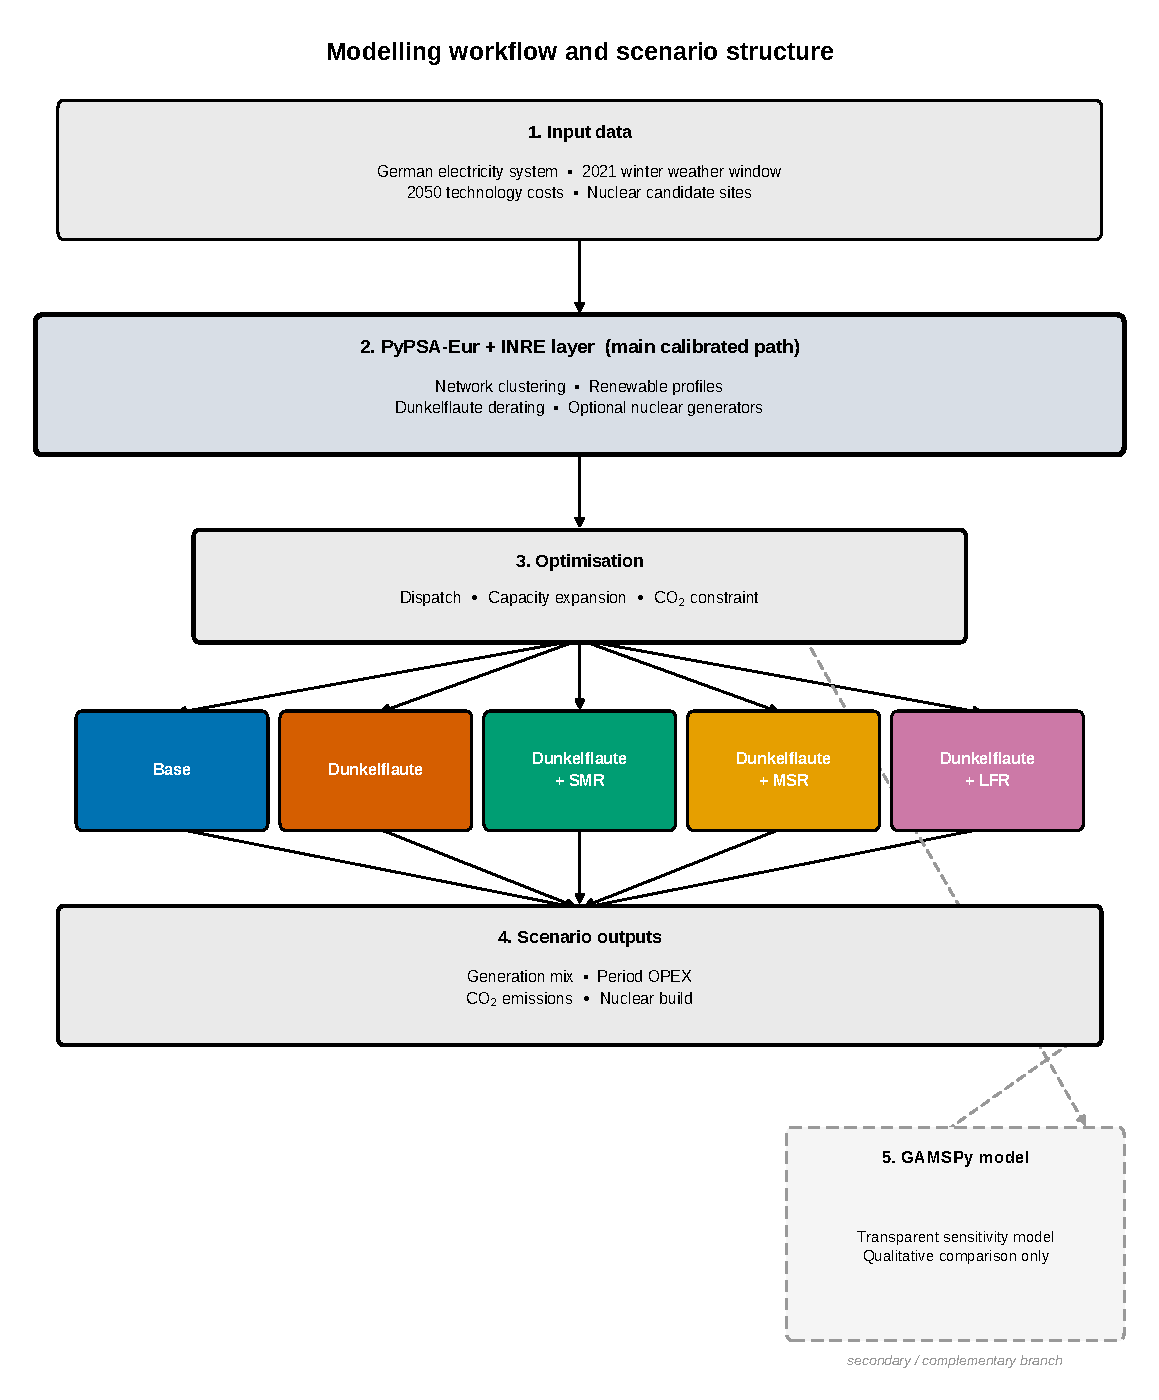
\includegraphics[width=0.85\textwidth]{figures/fig01_model_workflow_scenario_design.pdf}
    \caption{Modelling workflow used in the study. PyPSA-Eur with the INRE
    extension layer provides the main calibrated network-based results,
    while GAMSPy is used as a transparent complementary model for
    qualitative sensitivity checking. Input data (German electricity
    system, 2021 winter weather window, 2050 technology costs, nuclear
    candidate sites) feed the PyPSA-Eur~+~INRE layer, which handles network
    clustering, renewable profiles, Dunkelflaute derating, and optional
    nuclear generators. The optimisation stage (dispatch, capacity
    expansion, CO$_2$ constraint) is solved separately for each of the five
    scenarios (Base, Dunkelflaute, and Dunkelflaute with SMR, MSR, or LFR
    nuclear), producing the scenario outputs summarised in this report.}
    \label{fig:workflow}
\end{figure}

% ---------------------------------------------------------------------------
% Figure 2 — Dunkelflaute derating profile
% Full-width
% ---------------------------------------------------------------------------
\begin{figure}[htbp]
    \centering
    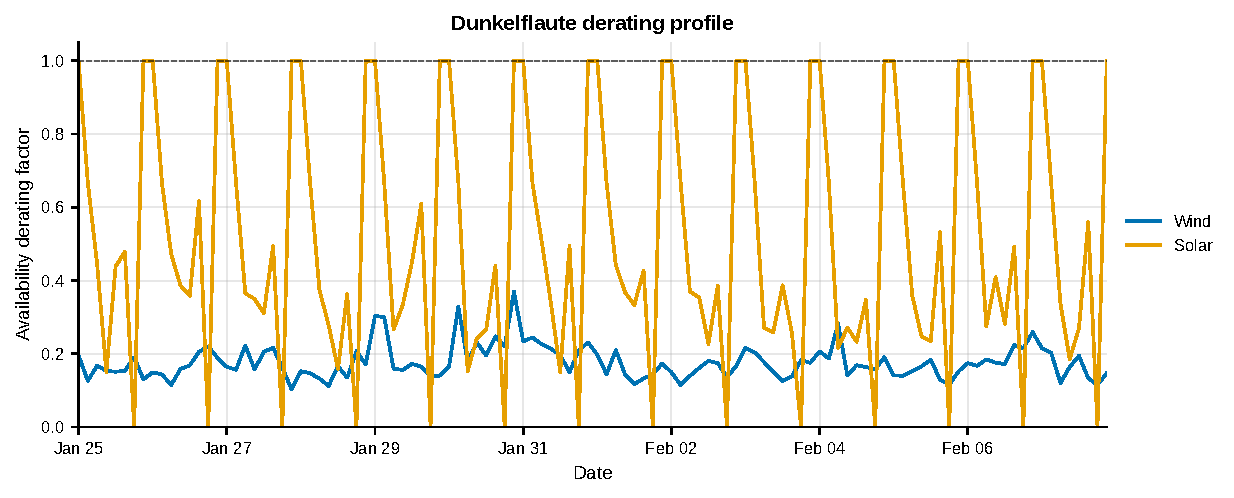
\includegraphics[width=\textwidth]{figures/fig02_dunkelflaute_derating_profile.pdf}
    \caption{Wind and solar availability derating factors applied during
    the 14-day Dunkelflaute stress window (25~January -- 7~February~2021,
    336~h, 3-hourly resolution). Values below one indicate reduced
    renewable availability relative to the baseline profile. This is a
    scenario \emph{input} figure: it characterises the imposed stress, not
    the resulting generation output (see Figure~\ref{fig:opresponse} for
    the operational response).}
    \label{fig:derating}
\end{figure}

% ---------------------------------------------------------------------------
% Figure 3 — Operational response to Dunkelflaute
% Single-column
% ---------------------------------------------------------------------------
\begin{figure}[htbp]
    \centering
    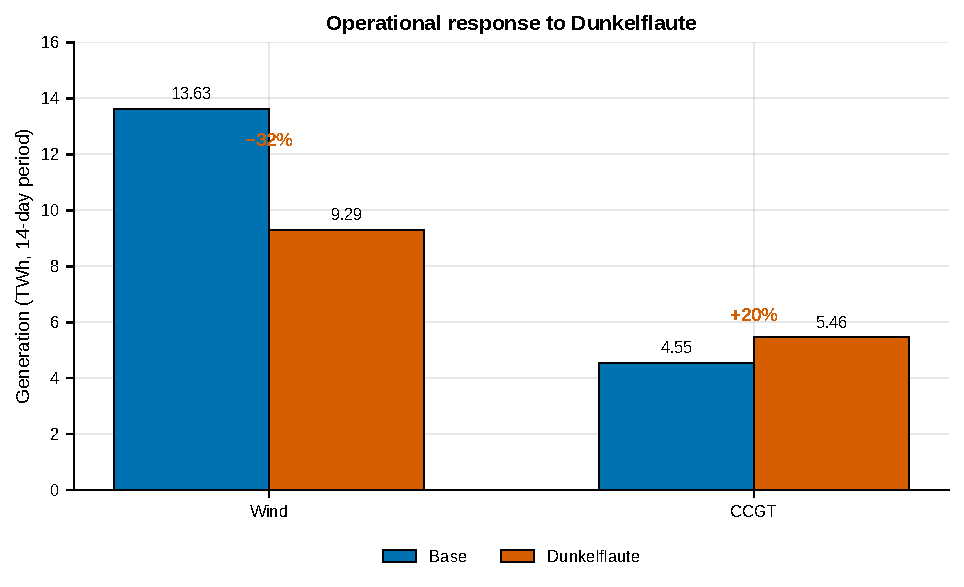
\includegraphics[width=0.85\columnwidth]{figures/fig03_dunkelflaute_operational_response.pdf}
    \caption{The main interpretable Dunkelflaute response is a 32\%
    reduction in wind generation (13.63 $\rightarrow$ 9.29~TWh) and a 20\%
    increase in CCGT generation (4.55 $\rightarrow$ 5.46~TWh) over the
    14-day simulation window, comparing the Base and Dunkelflaute
    scenarios. Solar is excluded from this comparison because
    main-scenario solar generation is not interpretable as a Dunkelflaute
    signal (profile mismatch and phantom capacity expansion in the main
    runs; see Figure~\ref{fig:fixedsolar} for the fixed-capacity
    sensitivity).}
    \label{fig:opresponse}
\end{figure}

% ---------------------------------------------------------------------------
% Figure 4 — Cost and emission impact of Dunkelflaute
% Full-width
% ---------------------------------------------------------------------------
\begin{figure}[htbp]
    \centering
    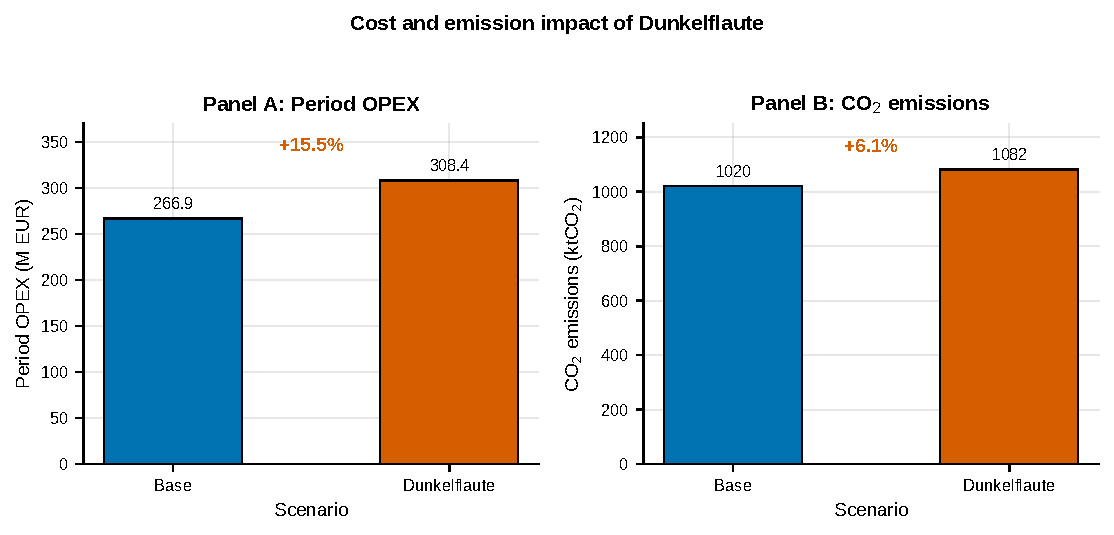
\includegraphics[width=\textwidth]{figures/fig04_opex_co2_impact.pdf}
    \caption{Dunkelflaute increases 14-day operating cost by 15.5\%
    (266.9 $\rightarrow$ 308.4~M~EUR period OPEX) and CO$_2$ emissions by
    6.1\% (1{,}020 $\rightarrow$ 1{,}082~ktCO$_2$), comparing the Base and
    Dunkelflaute scenarios. Cost is reported as period OPEX
    (\texttt{n.statistics.opex()}), not the solver objective or annuitised
    CAPEX, per the metric-selection rules in this report (annual CAPEX is
    never added to the 14-day OPEX figure). The CO$_2$ cap
    (50~Mt/yr $\rightarrow$ 1{,}918~ktCO$_2$ pro-rata) is non-binding in
    both runs, so CCGT remains available as the main balancing technology.}
    \label{fig:opexco2}
\end{figure}

% ---------------------------------------------------------------------------
% Figure 5 — Generation mix across scenarios
% Full-width
% ---------------------------------------------------------------------------
\begin{figure}[htbp]
    \centering
    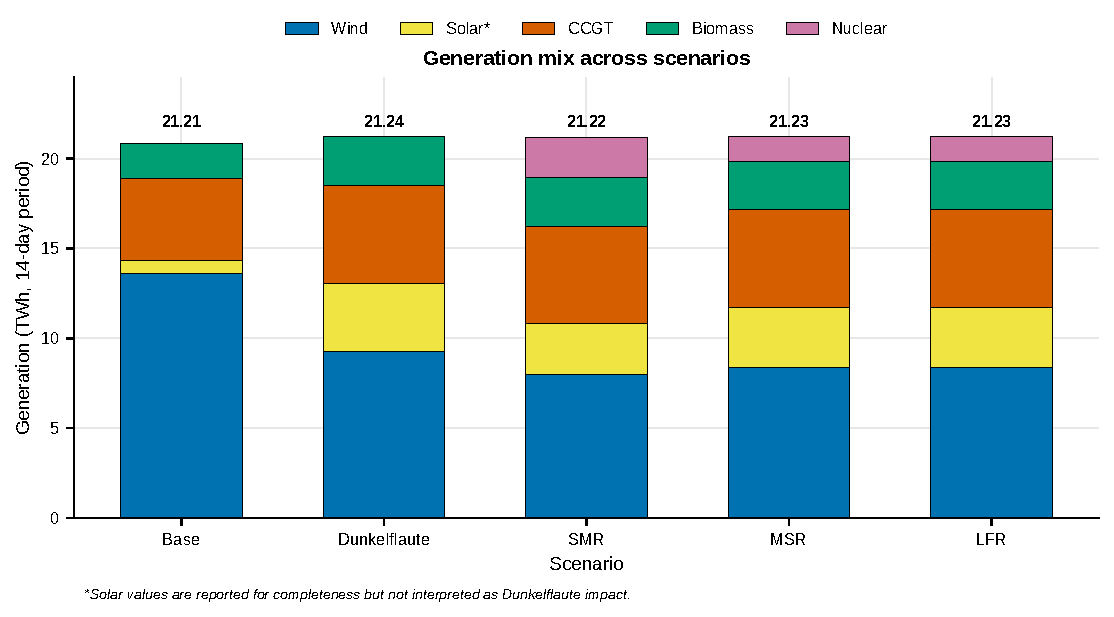
\includegraphics[width=\textwidth]{figures/fig05_generation_mix_by_scenario.pdf}
    \caption{Generation mix over the 14-day simulation window across all
    five scenarios (Base, Dunkelflaute, SMR, MSR, LFR). Wind reduction and
    the CCGT response are the main interpretable Dunkelflaute signals.
    Solar values (marked with an asterisk) are shown for completeness but
    are not used to infer the stress effect, owing to profile and
    phantom-capacity artefacts in the main scenario runs (Section~9 /
    Figure~\ref{fig:fixedsolar}). Nuclear generation appears only in the
    SMR, MSR, and LFR scenarios, reflecting endogenous builds to
    per-site capacity caps (Section~8); this is a model outcome under a
    2-week horizon and site constraints, not a deployment recommendation.}
    \label{fig:genmix}
\end{figure}

% ---------------------------------------------------------------------------
% Figure 6 — Interpretable capacity outcomes
% Full-width
% ---------------------------------------------------------------------------
\begin{figure}[htbp]
    \centering
    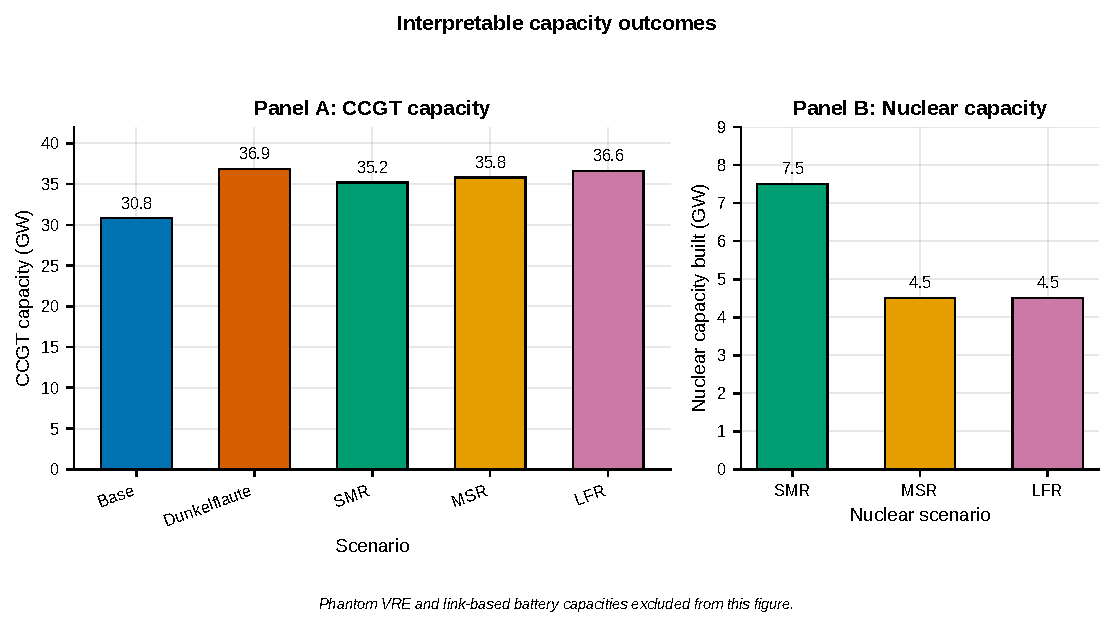
\includegraphics[width=\textwidth]{figures/fig06_credible_capacity_outcomes.pdf}
    \caption{Credible capacity indicators from the cleaned results. CCGT
    capacity expands under stress across all scenarios (Panel~A), while
    nuclear builds to per-site caps when enabled -- 7.5~GW for SMR and
    4.5~GW for MSR and LFR (Panel~B). Optimiser-reported phantom VRE
    (onshore wind up to 488~GW, solar up to 916~GW) and link-based battery
    capacities (up to 414~GW) are numerical artefacts of the short
    horizon and uncapped extendable carriers; they are excluded from this
    figure and from the main capacity interpretation (Appendix~A).}
    \label{fig:capacity}
\end{figure}

% ---------------------------------------------------------------------------
% Figure 7 — Nuclear output and CO2 effect
% Full-width
% ---------------------------------------------------------------------------
\begin{figure}[htbp]
    \centering
    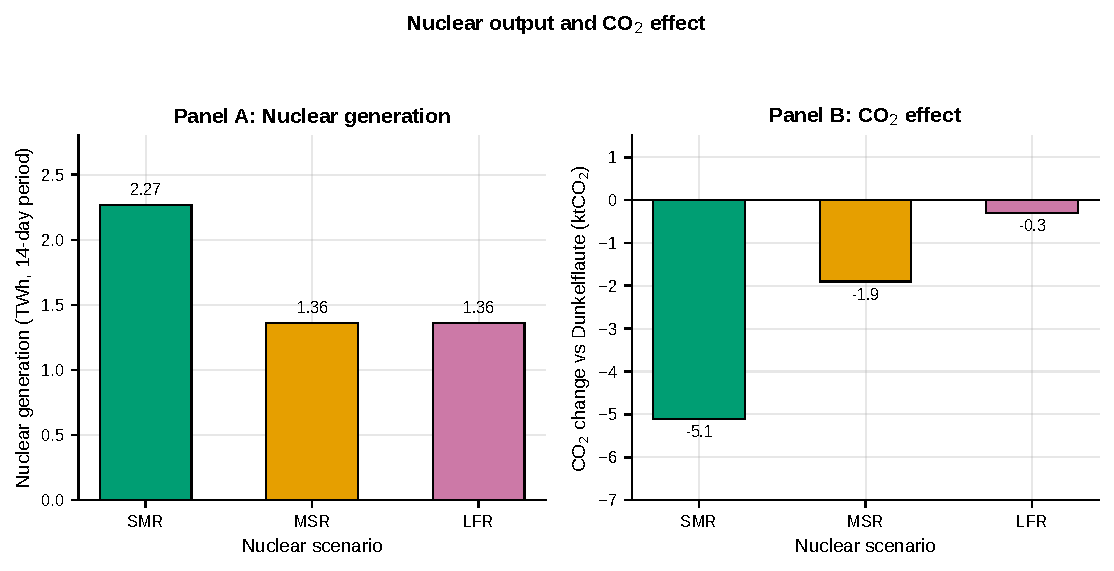
\includegraphics[width=\textwidth]{figures/fig07_nuclear_generation_and_co2_effect.pdf}
    \caption{Nuclear-enabled scenarios provide 1.36--2.27~TWh of firm
    generation over the 14-day period (Panel~A), but CO$_2$ reductions
    relative to the no-nuclear Dunkelflaute case remain below 10~ktCO$_2$
    in all three cases (Panel~B: $-$5.1~kt for SMR, $-$1.9~kt for MSR,
    $-$0.3~kt for LFR). Because this abatement is below the 10~ktCO$_2$
    threshold used in this report, it is not treated as policy-grade and
    abatement-cost (LCOA) figures are not headlined (Section~11). Nuclear
    supplies firm energy, but the associated CO$_2$ reduction remains
    marginal over this simulation window.}
    \label{fig:nuclearco2}
\end{figure}

% ---------------------------------------------------------------------------
% Figure 8 — Fixed-capacity stress sensitivity
% Full-width
% ---------------------------------------------------------------------------
\begin{figure}[htbp]
    \centering
    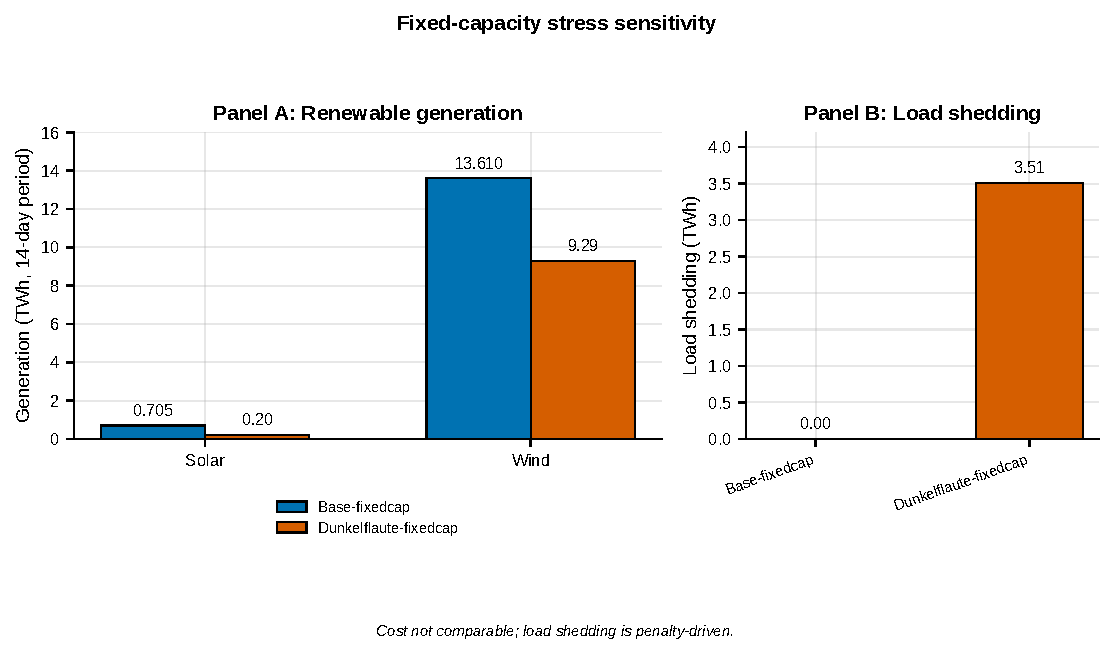
\includegraphics[width=\textwidth]{figures/fig08_fixed_solar_sensitivity.pdf}
    \caption{When solar capacity is fixed to the Base level, solar output
    falls under stress from 0.705~TWh to 0.203~TWh (Panel~A), confirming
    the expected physical direction that main-scenario solar results do
    not show. The stressed fixed-capacity run also reveals a 3.51~TWh
    adequacy gap through load shedding (Panel~B), but its cost
    ($\sim$35{,}450~M~EUR) is not comparable to the main scenarios because
    load shedding is penalty-priced rather than reflecting operational
    cost (Section~10).}
    \label{fig:fixedsolar}
\end{figure}

% ---------------------------------------------------------------------------
% Figure 9 — Worst-day dispatch under Dunkelflaute-SMR
% Single-column
% Note: generated from the daily-GWh fallback values (time-series
% generators_t.p extraction was not available in the figure-generation
% environment -- no pypsa / netCDF4 / network access). If a full 3-hourly
% stacked-area version is later produced from the network file, replace
% this figure and update the caption/axis units to GW.
% ---------------------------------------------------------------------------
\begin{figure}[htbp]
    \centering
    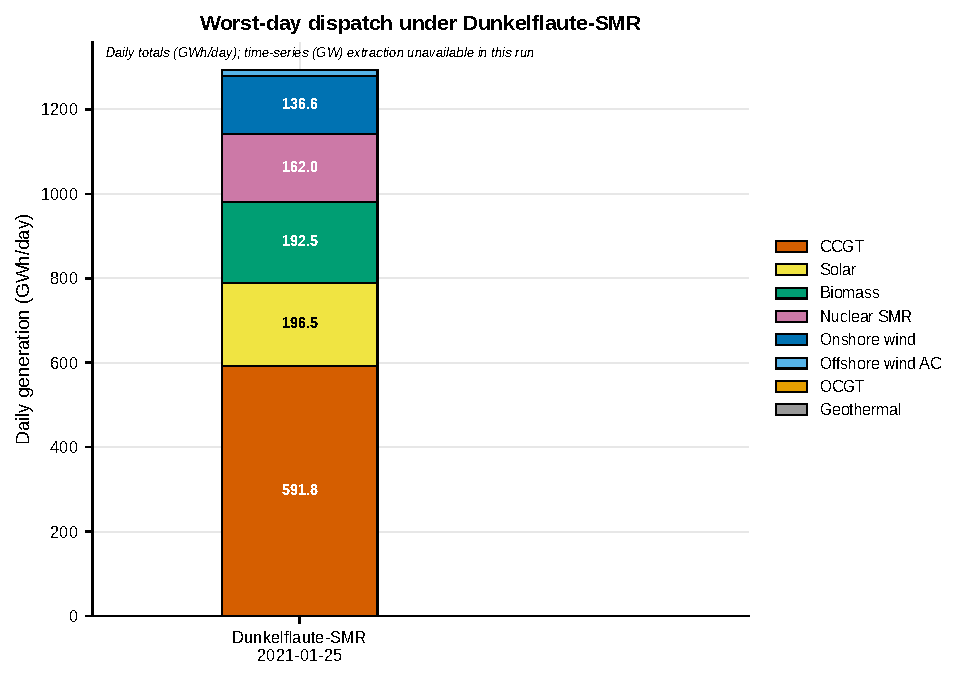
\includegraphics[width=0.85\columnwidth]{figures/fig09_worst_day_dispatch.pdf}
    \caption{Daily generation by carrier on 25~January~2021, the
    lowest-wind day within the Dunkelflaute-SMR scenario. CCGT remains the
    dominant source of daily generation (591.8~GWh/day), while SMR
    provides firm baseload output (162.0~GWh/day). Values are daily totals
    (GWh/day); a 3-hourly dispatch profile (GW) was not extracted for this
    figure.}
    \label{fig:worstday}
\end{figure}

% ---------------------------------------------------------------------------
% Figure 10 — Cross-model directional comparison
% Full-width
% ---------------------------------------------------------------------------
\begin{figure}[htbp]
    \centering
    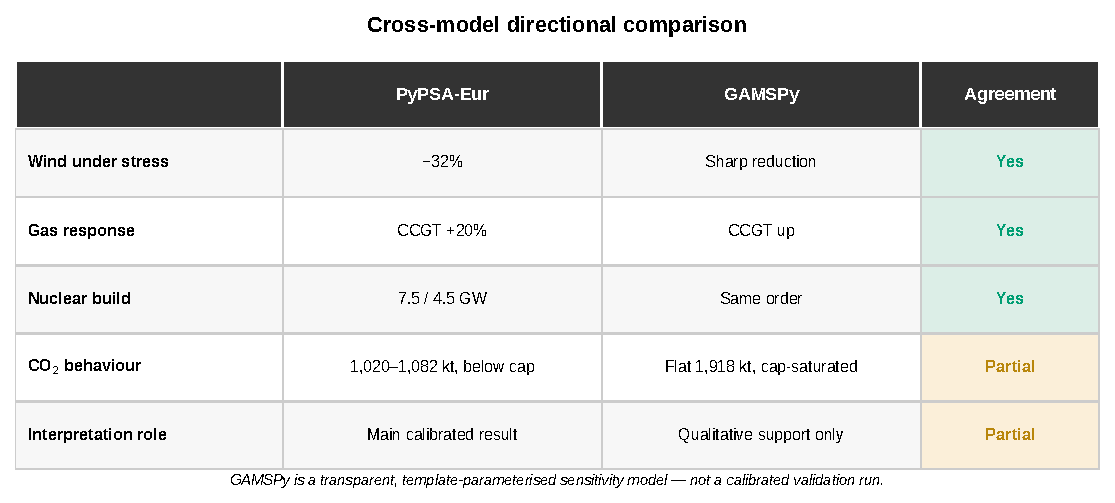
\includegraphics[width=\textwidth]{figures/fig10_pypsa_gamspy_directional_comparison.pdf}
    \caption{GAMSPy supports the main directional trends observed in
    PyPSA-Eur -- reduced wind under stress, increased gas dispatch, and
    nuclear building to the same order of magnitude -- but absolute costs
    and emission levels are not compared, because GAMSPy uses
    representative template inputs and simplified constraints rather than
    the calibrated PyPSA-Eur network. CO$_2$ behaviour and overall
    interpretation role show only partial agreement: GAMSPy's CO$_2$
    constraint saturates at the cap (1{,}918~ktCO$_2$), whereas PyPSA-Eur
    remains below it (1{,}020--1{,}082~ktCO$_2$). GAMSPy is used throughout
    this report as qualitative, directional support only, not as a
    calibrated validation of PyPSA-Eur results.}
    \label{fig:gamspy}
\end{figure}
